\chapter{Dimensionality Reduction}
In previous chapters covering supervised learning techniques, we often used basis functions to project our data into higher dimensions prior to applying an inference technique. This allowed us to construct more expressive models, which ultimately produced better results. While it may seem counterintuitive, in this chapter we're going to focus on doing exactly the opposite: reducing the dimensionality of our data through a technique known as Principle Component Analysis (PCA). We will also explore why it is necessary to reduce the dimensionality of some data sets.

\section{Motivation}
Real-world data is often very high dimensional, and it's common that our data sets contain features we are unfamiliar with, either because we are not a domain expert or because the dimensionality is too large for us to comb through the features by hand.

In these situations, it can be very difficult to manipulate or utilize our data effectively. We don't have a sense for which features are `important' and which ones are just noise. Fitting a model to the data may be computationally expensive, and even if we were to fit some sort of model to our data, it may be difficult to interpret why we obtain specific results. It's also hard to gain intuition about our data through visualization since humans struggle to think in more than three dimensions. All of these are good reasons that we may wish to reduce the dimensionality of a data set.

\begin{mlcube}{Dimensionality Reduction}
Dimensionality reduction operates primarily on continuous feature spaces, is fully unsupervised, and is non-probabilistic for the techniques we explore in this chapter.
\begin{center}
    \begin{tabular}{c|c|c}
    \textit{\textbf{Domain}} & \textit{\textbf{Training}} & \textit{\textbf{Probabilistic}} \\
    \hline
    Continuous & Unsupervised & No \\
    \end{tabular}
\end{center}
\end{mlcube}

While dimensionality reduction is considered an unsupervised technique, it might be better thought of as a tool used to make data more manageable prior to taking some other action. In fact, it's an important preprocessing step for a host of use cases.

\section{Applications}
As described above, we need a tool like dimensionality reduction in situations where high-dimensional data hinders us. Here are a few specific situations where we would use such a technique:

\begin{enumerate}
    \item Presenting differences between complex molecules in two dimensions (via a graph).
    \item Understanding the results of a credit trustworthiness algorithm.
    \item Efficiently training a neural network to predict supermarket sales on a data set with many input features.
    \item Identifying which costly measurements are worth collecting when experimenting with new chemicals.
\end{enumerate}

With a few of these use cases in mind, we now turn to the math that underpins the dimensionality reduction technique known as Priniciple Component Analysis.

\section{Principle Component Analysis}
The main idea behind Principle Component Analysis (PCA) is that we can linearly project our data set onto a subspace without losing too much information. For example, three-dimensional data might primarily exist in a subspace that is actually a two-dimensional plane.

One way to think about this is to identify and preserve the features along which there is the most variance. For example, imagine we had a data set comprised of the heights and weights of individual bears. As an extreme case, let's suppose all the bears were exactly the same height but had a wide range of weights.

\begin{figure}
    \centering
    \textbf{Bear Heights and Weights}\par\medskip
    
\includegraphics[width=0.5\paperwidth]{../DimensionalityReduction/fig/bear-graph.png}
    \caption{Graph of bear heights and weights.}
    \label{fig:bear-graph}
\end{figure}

To differentiate our data points, we obviously only need to report the weights of the bears. The variance of the heights is 0, and the variance of the weights is some non-zero number. Intuitively, the most interesting features from our data sets are those that vary the most.

\readernote{In this simple example, the direction of maximal variance occurs exactly along the $x_1$ axis, but in general it will occur on a plane described by a combination of our input features.}

The second way to think about PCA is that we are minimizing the error we incur when we move from the lower-dimensional representation back to the original representation. This is known as \textit{reconstruction loss}. We can consider the meaning of this using our bear example.

Let's say we project the data set from Figure \ref{fig:bear-graph} here down to a single dimension by recording only the weights:

\begin{figure}
    \centering
    \textbf{Bear Weights}\par\medskip
    
\includegraphics[width=0.5\paperwidth]{../DimensionalityReduction/fig/bear-weights-line.png}
    \caption{Bear weights.}
    \label{fig:bear-weights-line}
\end{figure}

Then, to reconstruct our original graph, we need only to keep track of a slope and bias term in the form of the familiar equation $x_2 = mx_1 + b$. In this case our slope is $m=0$ and our bias $b=3$. Note that this storage overhead is constant (just remembering the slope and bias) regardless of how big our data set gets. Thus we can go from our low-dimensional representation back to our original data:

\begin{figure}
    \centering
    \textbf{Converting Between Reduced and Original Data}\par\medskip
    
\includegraphics[width=0.5\paperwidth]{../DimensionalityReduction/fig/bear-conversion.png}
    \caption{Converting between the reduced data and original data.}
    \label{fig:bear-conversion}
\end{figure}

It will be our goal to determine a low-dimensional representation of our data that allows us to return to our high-dimensional data while losing as little information as possible. We wish to preserve everything salient about the data while discarding as much redundant information as possible. We now turn to how this can be achieved.

\subsection{Reconstruction Loss}
We identified a key tenet of dimensionality reduction in the previous section: finding subspaces of our data that preserve as much information as possible. Concretely, this means we want to convert our original data point $\textbf{x}_n$ in $D$ dimensions into a data point $\textbf{x}'_{n}$ in $D'$ dimensions where $D' < D$. 

\readernote{We're going to assume that our data set has been centered such that each feature in $\textbf{x}_{n}$ has mean 0. This will not affect our results (we can convert back to the uncentered data by adding back the mean of each feature), but will make our derivations more convenient to work with.}

Let's consider a simple case first: $D'=1$. This means that we're projecting our $D$ dimensional data down onto just a single dimension, or in geometric terms, we're projecting our data points $\textbf{x}_{n}$ onto a line through the origin. We can define this line as the unit vector $\textbf{w} \in \mathbb{R}^{D \times 1}$, and the projection is given by the dot product $\textbf{x} \cdot \textbf{w}$.

\readernote{The unit vector $\textbf{w}$ onto which we project our data is known as a \textit{principle component}, from which PCA gets its name.}

This projection produces a scalar, and that scalar defines how far our projection $\textbf{x} \cdot \textbf{w}$ is from the origin. We can convert this scalar back to $D$ dimensional space by multiplying it with the unit vector $\textbf{w}$. This means that $(\textbf{x} \cdot \textbf{w})\textbf{w}$ is the result of projecting our data point $\textbf{x}$ down into one-dimension and then converting it to its coordinate location in $D$ dimensions. We refer to these as our \textit{projection vectors}, and we can observe what this looks like geometrically in Figure \ref{fig:data-reconstruction}.

\begin{figure}
    \centering
    \textbf{Data Reconstruction}\par\medskip
    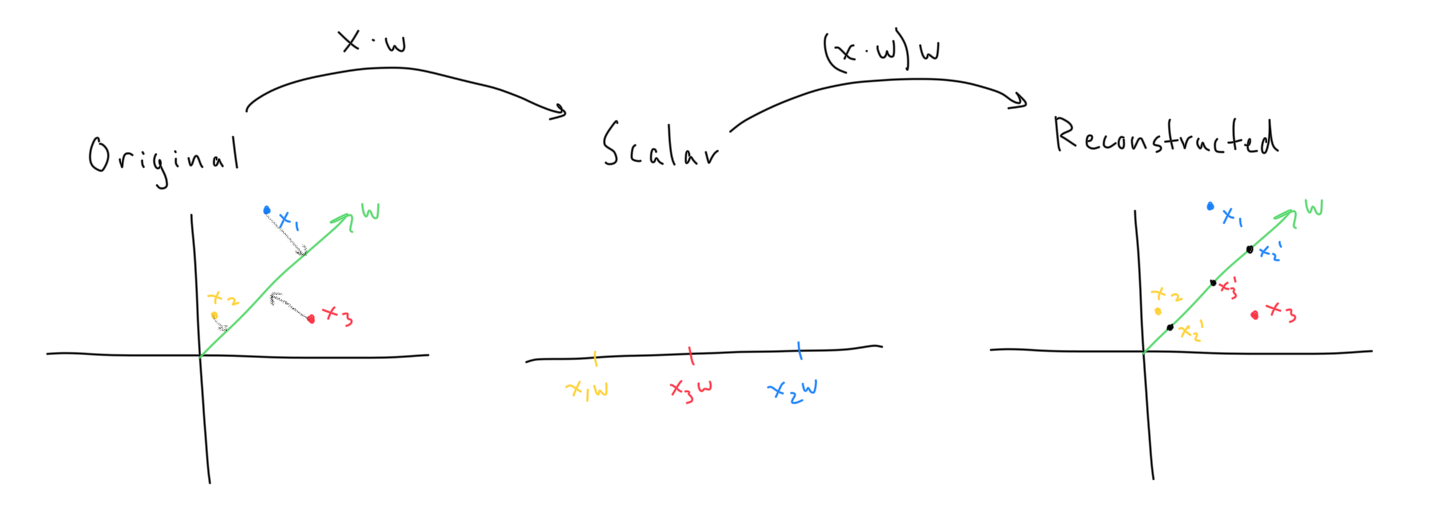
\includegraphics[width=0.5\paperwidth]{../DimensionalityReduction/fig/data-reconstruction.png}
    \caption{Far left: our original data. Middle: our reduced data in scalar form after the projection given by $\textbf{x} \cdot \textbf{w}$. Right: our reconstructed data points given by $(\textbf{x} \cdot \textbf{w})\textbf{w}$. Notice that our reconstructed data points are not the same as our original data.}
    \label{fig:data-reconstruction}
\end{figure}

The projection vectors we recover from the expression $(\textbf{x} \cdot \textbf{w})\textbf{w}$ will be in $D$ dimensions, but they will obviously not be identical to the original $D$ dimensional vectors (Figure \ref{fig:data-reconstruction} demonstrates why that is the case). This difference between the original and projection vectors can be thought of as error, since it is information lost from our original data. For a given data point $\textbf{x}_{n}$ and unit vector $\textbf{w}$, we can measure this error through the expression:
\begin{equation} \label{reconstruction-loss}
	||\textbf{x}_{n} - (\textbf{x} \cdot \textbf{w})\textbf{w}||^{2}
\end{equation}
which is known as \textbf{reconstruction loss} because it measures the error incurred when reconstructing our original data from its projection. 

\begin{definition}{Reconstruction Loss}{reconstruction-loss}
    Reconstruction loss is the difference (measured via a distance metric such as Euclidean distance) between an original data set and its reconstruction from a lower dimensional representation. It indicates how much information is lost during dimensionality reduction.
\end{definition}

Reconstruction loss is then a metric for evaluating how `good' a subspace in $D'$ dimensions is at representing our original data in $D$ dimensions. The better it is, the less information we lose, and the reconstruction loss is lower as a result.

\subsection{Minimizing Reconstruction Loss}
We now know that our goal is to find a good subspace to project onto, and we also know that finding this good subspace is equivalent to minimizing the reconstruction loss it incurs. We can now formalize this as an optimization problem.

First, we simplify the reconstruction loss for a single data point $\textbf{x}_n$ as follows:
\begin{align*}
	||\textbf{x}_{n} - (\textbf{x}_{n} \cdot \textbf{w})\textbf{w}||^{2} &= (\textbf{x}_{n} - (\textbf{x}_{n} \cdot \textbf{w})\textbf{w})(\textbf{x}_{n} - (\textbf{x}_{n} \cdot \textbf{w})\textbf{w}) \\
	&= ||\textbf{x}_{n}||^{2} - 2(\textbf{x}_{n} \cdot \textbf{w})^{2} + (\textbf{x}_{n} \cdot \textbf{w})^{2}||\textbf{w}||^{2} \\
	&= ||\textbf{x}_{n}||^{2} - (\textbf{x}_{n} \cdot \textbf{w})^{2} \\
\end{align*}
where $||\textbf{w}||^{2} = 0$ because it is a unit vector. Note that we can define reconstruction loss over our entire data set as follows:
\begin{equation} \label{full-reconstruction-loss}
    RL(\textbf{w}) = \frac{1}{n} \sum_{n=1}^{N} ||\textbf{x}_{n}||^{2} - (\textbf{x}_{n} \cdot \textbf{w})^{2} \\
\end{equation}
Recall that our goal is to minimize reconstruction loss over our data set by optimizing the subspace defined by $\textbf{w}$. Let's first rewrite Equation \ref{full-reconstruction-loss} as:
\begin{align*}
    RL(\textbf{w}) = \frac{1}{n} \sum_{n=1}^{N} ||\textbf{x}_{n}||^{2} - \frac{1}{n} \sum_{n=1}^{N} (\textbf{x}_{n} \cdot \textbf{w})^{2} \\
\end{align*}
where we can see that our optimization will depend only on maximizing the second term:
\begin{equation} \label{max-for-recon-loss}
    \frac{1}{n} \sum_{n=1}^{N} (\textbf{x}_{n} \cdot \textbf{w})^{2}
\end{equation}
since it is the only one involving \textbf{w}. Recall that the sample mean of a data set is given by the expression $\frac{1}{n} \sum_{n=1}^{N} \textbf{x}_{n}$, and note that Equation \ref{max-for-recon-loss} is the sample mean of $(\textbf{x} \cdot \textbf{w})^{2}$. Using the definition of variance for a random variable $\textbf{Z}$ (which is given by $Var(\textbf{Z}) = \mathbb{E}(\textbf{Z}^{2}) - (\mathbb{E}(\textbf{Z}))^{2}$), we can rewrite Equation \ref{max-for-recon-loss} as:
\begin{align*}
    \frac{1}{n} \sum_{n=1}^{N} (\textbf{x}_{n} \cdot \textbf{w})^{2} &= Var\big[\{\textbf{x}_{n} \cdot \textbf{w}\}_{n=1}^{N}\big] + \big( \mathbb{E} \big[\{\textbf{x}_{n} \cdot \textbf{w}\}_{n=1}^{N}\big] \big)^{2}
\end{align*}
Recall that we centered our data $\textbf{x}_{n}$ to have mean 0 such that the expression above simplifies to:
\begin{equation} \label{variance-equivalence}
    \frac{1}{n} \sum_{n=1}^{N} (\textbf{x}_{n} \cdot \textbf{w})^{2} = Var\big[\{\textbf{x}_{n} \cdot \textbf{w}\}_{n=1}^{N}\big] \\
\end{equation}
and therefore $Var\big[\{\textbf{x}_{n} \cdot \textbf{w}\}_{n=1}^{N}\big]$ is the term we wish to maximize. \textbf{This means that minimizing the reconstruction loss is equivalent to maximizing the variance of our projections $\{\textbf{x}_{n} \cdot \textbf{w}\}_{n=1}^{N}$}.

\readernote{Note the intuitiveness of this result. We should like to find a subspace that maintains the spread in our data.}

\subsection{Multiple Principle Components}
Up until now, we've been considering how we would project onto a single principle component $\textbf{w} \in \mathbb{R}^{D \times 1}$. This will reduce our data down to one dimension, just a scalar. In general, we will wish to preserve more of our data than just a single dimension, which means that we will need to have multiple principal components. For now we'll assume that our principal components are orthogonal (we will prove this later), which then allows us to describe the projection of our data $\textbf{x}_{n}$ onto this subspace as the sum of the projections onto $D'$ orthogonal vectors:
\begin{equation} \label{orthogonal-projections}
    \sum_{d'=1}^{D'} (\textbf{x}_{n} \cdot \textbf{w}_{d'})\textbf{w}_{d'}
\end{equation}

\subsection{Identifying Directions of Maximal Variance in our Data}
We now know from the previous section that we find our principle components (and thus the subspace we will project onto) by identifying the directions of maximum variance in our projected data set. We know from Equation \ref{variance-equivalence} that the variance is equivalent to:
\begin{equation*}
    \sigma^{2}_{\textbf{w}} \equiv Var\big[\{\textbf{x}_{n} \cdot \textbf{w}\}_{n=1}^{N}\big] = \frac{1}{n} \sum_{n=1}^{N} (\textbf{x}_{n} \cdot \textbf{w})^{2}
\end{equation*}
Rewriting this in terms of matrix notation we have that:
\begin{equation*}
    \sigma^{2}_{\textbf{w}} = \frac{1}{n} (\textbf{X} \textbf{w})^{T} (\textbf{X} \textbf{w})
\end{equation*}
We can further simplify this:
\begin{align*}
    \sigma^{2}_{\textbf{w}} &= \frac{1}{n} \textbf{w}^{T}\textbf{X}^{T} \textbf{X} \textbf{w} \\
    \sigma^{2}_{\textbf{w}} &= \frac{1}{n} \textbf{w}^{T}\textbf{X}^{T} \textbf{X} \textbf{w} \\
    \sigma^{2}_{\textbf{w}} &= \textbf{w}^{T} \frac{\textbf{X}^{T}\textbf{X}}{n} \textbf{w} \\
    \sigma^{2}_{\textbf{w}} &= \textbf{w}^{T} \textbf{S} \textbf{w} \\
\end{align*}
where $\textbf{S} = \frac{\textbf{X}^{T}\textbf{X}}{n}$ is the empirical covariance matrix of our data set.

\readernote{Notice that by convention we describe the empirical covariance of a data set with the term $\textbf{S}$ instead of the usual covariance term $\Sigma$.}

Our goal is to maximize the term $\sigma^{2}_{\textbf{w}} = Var\big[\{\textbf{x}_{n} \cdot \textbf{w}\}_{n=1}^{N}\big]$ with respect to $\textbf{w}$. Furthermore, $\textbf{w}$ is a unit vector, so we must optimize subject to the constraint $\textbf{w}^{T}\textbf{w} = 1$. Recalling the discussion of Lagrange multipliers from Chapter 6 on Support Vector Machines, we incorporate this constraint by reformulating our optimization problem as the Lagrangian equation:
\begin{align*}
    \mathcal{L}(\textbf{w}, \lambda) &= \textbf{w}^{T} \textbf{S} \textbf{w} - \lambda(\textbf{w}^{T}\textbf{w} - 1) \\
\end{align*}
As usual, we proceed by taking the derivative with respect to each parameter:
\begin{align*}
    \frac{d\mathcal{L}(\textbf{w}, \lambda)}{d\textbf{w}} &= 2\textbf{S} \textbf{w} - 2\lambda\textbf{w} \\
    \frac{d\mathcal{L}(\textbf{w}, \lambda)}{d\lambda} &= \textbf{w}^{T}\textbf{w} - 1 \\
\end{align*}
We can now set these equal to 0 and solve for the optimal values:
\begin{align*}
    \textbf{S} \textbf{w} &= \lambda\textbf{w} \\
    \textbf{w}^{T}\textbf{w} &= 1 \\
\end{align*}
This result is very significant! As we knew already, we needed $\textbf{w}$ to be a unit vector. However, we also see that $\textbf{w}$ is an eigenvector of the empirical covariance matrix $\textbf{w}$. Futhermore, the eigenvector that will maximize our quantity of interest $\sigma^{2}_{\textbf{w}} = \textbf{w}^{T} \textbf{S} \textbf{w}$ will be the eigenvector with the largest eigenvalue $\lambda$. Fortunately, linear algebra gives us many tools for finding eigenvectors, and as a result we can efficiently identify our principal components. Note also that the eigenvectors of a symmetric matrix are orthogonal, which proves our earlier assumption that our principal components are orthogonal.

To recap, we've learned that the optimal principal components (meaning the vectors describing our projection subspace) are the eigenvectors of the empirical covariance matrix of our data set. The vector preserving the most variance in our data (and thus minimizing the reconstruction loss) is given by the eigenvector with the largest eigenvalue, followed by the eigenvector with the next largest eigenvalue, and so on. Furthermore, while it is somewhat outside the scope of this textbook, we are guaranteed to have $D$ distinct, orthogonal eigenvectors with eigenvalues $\geq 0$. This is a result of linear algebra that hinges on the fact that our empirical covariance matrix $\textbf{S}$ is symmetric and positive semi-definite.

\subsection{Choosing the Optimal Number of Principal Components}
We now know that the eigenvectors of the empirical covariance matrix $\textbf{S}$ give us the principal components that form our projection subspace. Note that the exact procedure for finding these eigenvectors is a topic better suited for a book on linear algebra, but if you are interested, you can look into a topic known as Singular Value Decomposition (SVD). For our purposes, we will assume there is a black box that accepts $\textbf{S}$ and returns a list of the $D$ principal components.

Because these principal components are orthogonal, the projections they produce will be entirely uncorrelated. This means we can project our original data onto each component individually and then sum those projections to create our lower dimensional data points. Note that it doesn't make sense that we would use every one of our $D$ principal components to define our projection subspace, since that wouldn't lead to a reduction in the dimensionality of our data at all (the $D$ orthogonal principal components span the entire $D$ dimensional space of our original data set). We now need to decide how many principal components we will choose to include, and therefore what subspace we will be projecting onto.

The `right' number of principal components to use depends on our goals. For example, if we simply wish to visualize our data, then we would project onto a 2D or 3D space. Therefore, we would choose the first 2 or 3 principal components, and project our original data onto the subspace defined by those vectors. This might look something like Figure \ref{fig:dim-red-iris}.

\begin{figure}
    \centering
    \textbf{Four Dimensional Iris Data Set in Three Dimensions}\par\medskip
    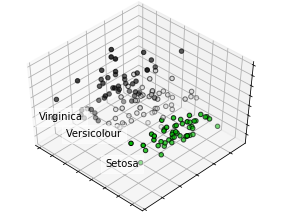
\includegraphics[width=0.5\paperwidth]{../DimensionalityReduction/fig/dim-red-iris.png}
    \caption{PCA applied to Fisher's Iris data set, which is originally in four dimensions. We reduce it to three dimensions for visualization purposes and label the different flower types. This example is taken from the sklearn documentation.}
    \label{fig:dim-red-iris}
\end{figure}

However, it's more complicated to choose the optimal number of principal components when our goal is not simply visualization. We're now left with the task of trading off how much dimensionality reduction we wish to achieve with how much information we want to preserve in our data.

One way to do this is similar to the informal `elbow' method described for K-Means clustering. We graph our reconstruction loss against the number of principal components used, as seen in Figure \ref{fig:RL-vs-PC}. The idea is to add principal components to our subspace one at a time, calculating the reconstruction loss as we go. The first few principal components will greatly reduce the reconstruction loss, before eventually leveling off. We can identify the `elbow' where the reduction in loss starts to diminish, and choose to use that number of principal components.

\begin{figure}
    \centering
    \textbf{Reconstruction Loss vs. Number of Principal Components}\par\medskip
    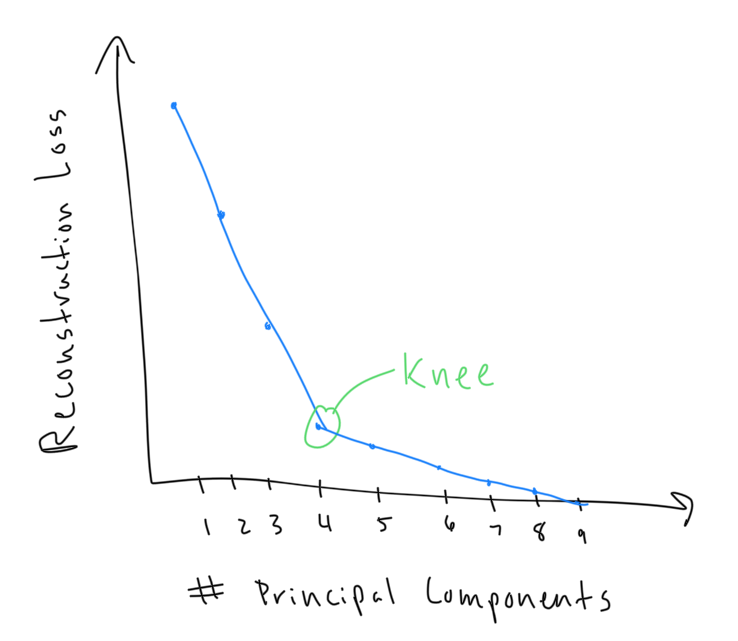
\includegraphics[width=0.5\paperwidth]{../DimensionalityReduction/fig/RL-vs-PC.png}
    \caption{Reconstruction loss versus the number of principal components. Notice the similarity to the `elbow' method of K-Means clustering.}
    \label{fig:RL-vs-PC}
\end{figure}

Another way to do this is to consider how much variance we wish to preserve in our data. Each principal component is associated with an eigenvalue $\lambda_{d}$ that indicates what proportion of the variance that principal component is responsible for in our data set. Then the fraction of variance retained from our data set if we choose to keep $D'$ principal components is given by:
\begin{equation} \label{variance-retention}
    \text{retained variance} = \frac{\sum_{d'=1}^{D'} \lambda_{d'}}{\sum_{d=1}^{D} \lambda{d}}
\end{equation}
For different applications, there may be different levels of acceptable variance retention, which can help us decide how many principal components to keep.

Finally, once we have selected our principal components, we have also defined the subspace onto which we will be projecting our original data. And although this subspace is defined by the basis given by our principal components, these principal components are not a unique description of that subspace. We could choose to use any basis after we've identified our subspace through the principal components. The importance of this idea is simply that although our principal components are unique, they are not the only basis we could use to define the same projection subspace.

\section{Conclusion}
Principal component analysis is useful for visualization purposes, removing redundant information, or making a data set more computationally manageable. PCA is also a good tool for data exploration, particularly when digging into an unfamiliar data set for the first time.

It is not essential that we know by heart the exact derivation for arriving at the principal components of a data set. The same can be said of the linear algebra machinery needed to compute principal components. However, it is important to have an intuitve grasp over how variance in our data set relates to principal components, as well as an understanding of how subspaces in our data can provide compact representations of that data set. These are critical concepts for working effectively with real data, and they will motivate related techniques in machine learning.